\subsection{MVM algorithm}

The \definition{Matrix-Vector Multiply (MVM) algorithm} consists of four steps:
\begin{enumerate}
    \item \textbf{Concurrent read of vector} $X\left(1 : n\right)$ (transfer $N$ elements);

    \item \textbf{Simultaneous reads of different sections of the general matrix} $A$ (transfer $\dfrac{n^{2}}{p}$ elements to each processor);

    \item \textbf{Compute} $\dfrac{n^{2}}{p}$ operations per processor;

    \item \textbf{Simultaneous writes} (transfer $\dfrac{n}{p}$ elements from each processor).
\end{enumerate}
Let $i$ be the processor index, so the MVM algorithm is simply written as:
\begin{lstlisting}[mathescape=true, caption={Matrix-Vector Multiply (MVM)}]
GLOBAL READ (Z $\leftarrow$ X)
GLOBAL READ (B $\leftarrow A_{i}$)
COMPUTE (W := BZ)
GLOBAL WRITE (W $\rightarrow y _{i}$)
\end{lstlisting}

\highspace
\begin{figure}[!htp]
    \centering
    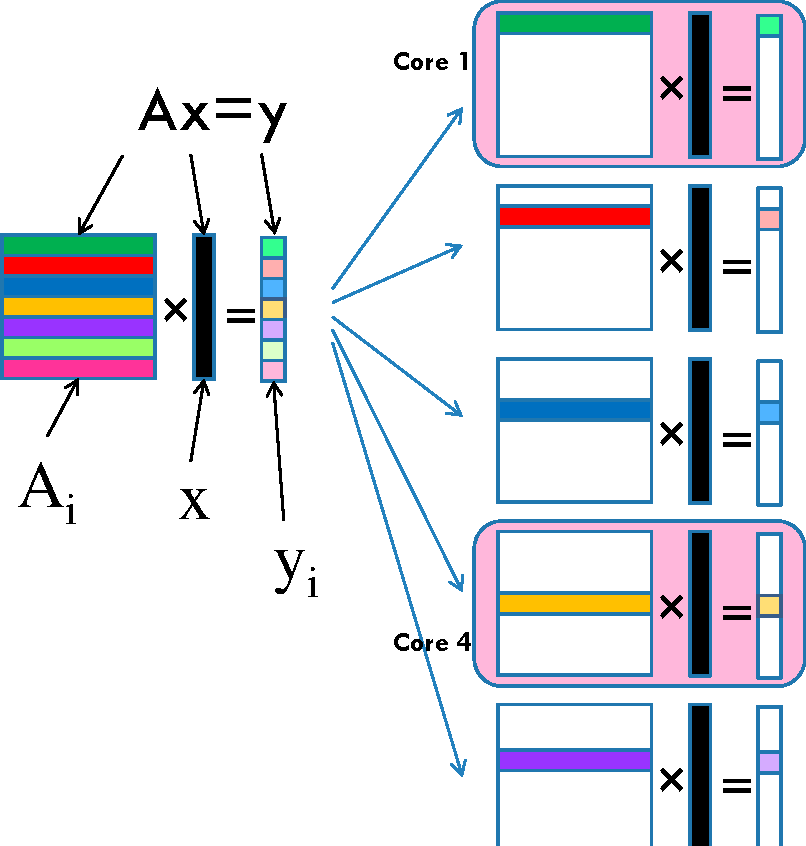
\includegraphics[width=.7\textwidth]{img/mvm-1.pdf}
    \caption{Example of MVM algorithm.}
\end{figure}

\newpage

\noindent
The performance of the MVM algorithm is as follows:
\begin{itemize}
    \item The \textbf{time to solve} a problem of size $n^{2}$ is equal to the big $O$ of the squared size of the problem as input divided by the number of processors available:
    \begin{equation*}
        T_{p}\left(n^{2}\right) = O\left(\dfrac{n^{2}}{p}\right)
    \end{equation*}
    
    \item The \textbf{cost} is equal to the number of processors and the time it takes to solve the problem. So it is quite trivial:
    \begin{equation*}
        C = O\left(\cancel{P} \cdot \dfrac{n^{2}}{\cancel{p}}\right) = O\left(n^{2}\right)
    \end{equation*}

    \item The \textbf{work} is equal to the cost, and the \textbf{linear power} $P$ is equal to the ratio of work and time to solve the problem on $p$ processors:
    \begin{equation*}
        W = C \hspace{2em} \dfrac{W}{T_{p}} = P
    \end{equation*}

    \item The \textbf{perfect efficiency} is equal to:
    \begin{equation*}
        E_{p} = \dfrac{T_{1}}{pT_{p}} = \dfrac{n^{2}}{p\frac{n^{2}}{p}} = 1
    \end{equation*}
\end{itemize}